\subsection{Conventions}

\subsubsection{Coordinate System} \label{sec:conv:coord}

Where coordinates are used, the cameras coordinate system is used. This means that, in an image frame from the camera's
perspective, the y-axis points up, the x-axis points left, and the z-axis extends into the depth dimension. 
This is illustrated in Fig. \ref{fig:coordinates}.

\begin{figure}[H]
    \centering
    \tdplotsetmaincoords{65}{115}
    \begin{tikzpicture}[tdplot_main_coords, scale=1.2, >=Stealth, line join=round] 
    %===================================================
    % Coordinate axes (camera frame: y up, z out of lens).
    % NOTE: to get y rendered as the vertical (up) axis with
    % these view angles, a *true* coordinate (X,Y,Z) is drawn
    % at the local pgf coordinate (X,Z,Y) throughout this
    % picture -- i.e. slot 2 <-> true z (depth), slot 3 <->
    % true y (height).
    %===================================================
    \draw[thick,-{Stealth[length=3mm]}] (0,0,0) -- (-1.5,0,0) node[above right]{$x$};
    \draw[thick,-{Stealth[length=3mm]}] (0,0,0) -- (0,0,1.5) node[above]{$y$};
    \draw[thick,-{Stealth[length=3mm]}] (0,0,0) -- (0,1.5,0) node[below right]{$z$};
    \filldraw[black] (0,0,0) circle (0.02);
    
    %===================================================
    % Vertical rod, parallel to the y axis, passing through
    % the z axis at some positive depth
    %===================================================
    \pgfmathsetmacro{\rodz}{2.6}
    \draw[ultra thick, black!60, line cap=round]
        (0,\rodz,-1.4) -- (0,\rodz,1.4);
    \filldraw[black!60] (0,\rodz,-1.4) circle (0.03);
    \filldraw[black!60] (0,\rodz, 1.4) circle (0.03);
    \node[anchor=west] at (0,\rodz,1.55) {Perch};
    
    %===================================================
    % Simple stereo camera, sitting on the negative z axis,
    % looking down the +z direction
    %===================================================
    \pgfmathsetmacro{\camz}{-1.8}
    
    % camera body (a flat box in the x-y plane at depth z = \camz)
    \draw[fill=black!75, draw=black]
        (-0.75,\camz,-0.3) -- (0.75,\camz,-0.3) --
        (0.75, \camz, 0.3) -- (-0.75, \camz, 0.3) -- cycle;
    
    % two lenses, offset along x (stereo baseline).
    % "circle" always draws in the flat, screen-facing canvas plane,
    % so it must be re-anchored into the camera body's own plane
    % (fixed local y = \camz, varying local x/z) via a canvas scope.
    \begin{scope}[canvas is xz plane at y=\camz]
        \filldraw[fill=black!40, draw=black] (-0.38,0) circle (0.2);
        \filldraw[fill=black!40, draw=black] ( 0.38,0) circle (0.2);
        \filldraw[fill=black]                (-0.38,0) circle (0.07);
        \filldraw[fill=black]                ( 0.38,0) circle (0.07);
    \end{scope}
    
    % dashed line showing the camera's viewing (+z) direction
    \draw[dashed, gray] (0,\camz,0) -- (0,0,0);
    
    \node[anchor=north] at (0,\camz,-0.45) {Stereo Camera};
    \end{tikzpicture}
    \caption{Illustration of coordinate conventions used in this thesis, where the z-axis extends
    outward from the cameras focal point and the y-axis extends vertically in the cameras frame.
    The illustration shows a test setup with the camera on the left and a test perch being detected
    on the right.}
    \label{fig:coordinates}
\end{figure}

\subsubsection{Measurements} \label{sec:conv:meas}

There are 3 position measurements relevant for the perch detection 
in this thesis:
\begin{itemize}
    \item Distance: $d$, distance along the z-axis between the camera and test object. Illustrated in Fig. \ref{fig:distance}
    \item Azimuth: $\alpha$, Angle between the y-axiz and the test object. Illustrated in Fig. \ref{fig:angles}
    \item Elevation: $\theta$, Angle between the x-y plane and the test object. Illustrated in Fig. \ref{fig:angles}
\end{itemize}

\begin{figure}[H]
    \centering
    \tdplotsetmaincoords{65}{115}
    \begin{tikzpicture}[tdplot_main_coords, scale=1.2, >=Stealth, line join=round] 
    %===================================================
    % Coordinate axes (camera frame: y up, z out of lens).
    % NOTE: to get y rendered as the vertical (up) axis with
    % these view angles, a *true* coordinate (X,Y,Z) is drawn
    % at the local pgf coordinate (X,Z,Y) throughout this
    % picture -- i.e. slot 2 <-> true z (depth), slot 3 <->
    % true y (height).
    %===================================================
    \draw[thick,-{Stealth[length=3mm]}] (0,0,0) -- (-1.5,0,0) node[above right]{$x$};
    \draw[thick,-{Stealth[length=3mm]}] (0,0,0) -- (0,0,1.5) node[above]{$y$};
    \draw[thick,-{Stealth[length=3mm]}] (0,0,0) -- (0,1.5,0) node[below right]{$z$};
    \filldraw[black] (0,0,0) circle (0.02);
    
    %===================================================
    % Vertical rod, parallel to the y axis, passing through
    % the z axis at some positive depth
    %===================================================
    \pgfmathsetmacro{\rodz}{2.6}
    \draw[ultra thick, black!60, line cap=round]
        (0,\rodz,-1.4) -- (0,\rodz,1.4);
    \filldraw[black!60] (0,\rodz,-1.4) circle (0.03);
    \filldraw[black!60] (0,\rodz, 1.4) circle (0.03);
    \node[anchor=west] at (0,\rodz,1.55) {Perch};
    
    %===================================================
    % Simple stereo camera, sitting on the negative z axis,
    % looking down the +z direction
    %===================================================
    \pgfmathsetmacro{\camz}{-1.8}
    
    % camera body (a flat box in the x-y plane at depth z = \camz)
    \draw[fill=black!75, draw=black]
        (-0.75,\camz,-0.3) -- (0.75,\camz,-0.3) --
        (0.75, \camz, 0.3) -- (-0.75, \camz, 0.3) -- cycle;
    
    % two lenses, offset along x (stereo baseline).
    % "circle" always draws in the flat, screen-facing canvas plane,
    % so it must be re-anchored into the camera body's own plane
    % (fixed local y = \camz, varying local x/z) via a canvas scope.
    \begin{scope}[canvas is xz plane at y=\camz]
        \filldraw[fill=black!40, draw=black] (-0.38,0) circle (0.2);
        \filldraw[fill=black!40, draw=black] ( 0.38,0) circle (0.2);
        \filldraw[fill=black]                (-0.38,0) circle (0.07);
        \filldraw[fill=black]                ( 0.38,0) circle (0.07);
    \end{scope}
    
    % dashed line showing the camera's viewing (+z) direction
    \draw[dashed, gray] (0,\camz,0) -- (0,0,0);

    % dashed line showing the distance measurement
    \draw[dashed, red] (0,\camz,-1) -- (0,\rodz,-1) node[midway,below,red]{d};
    
    \node[anchor=north] at (0,\camz,-0.45) {Stereo Camera};
    \end{tikzpicture}
    \caption{Illustration of the distance measurement from the stereo camera to the perch.}
    \label{fig:distance}
\end{figure}

\begin{figure}[H]
    \centering
    \tdplotsetmaincoords{65}{115}
    \begin{tikzpicture}[tdplot_main_coords, scale=1.2, >=Stealth, line join=round] 
    %===================================================
    % Coordinate axes (camera frame: y up, z out of lens).
    % NOTE: to get y rendered as the vertical (up) axis with
    % these view angles, a *true* coordinate (X,Y,Z) is drawn
    % at the local pgf coordinate (X,Z,Y) throughout this
    % picture -- i.e. slot 2 <-> true z (depth), slot 3 <->
    % true y (height).
    %===================================================
    \draw[thick,-{Stealth[length=3mm]}] (0,0,0) -- (-1.5,0,0) node[above right]{$x$};
    \draw[thick,-{Stealth[length=3mm]}] (0,0,0) -- (0,0,1.5) node[above]{$y$};
    \draw[thick,-{Stealth[length=3mm]}] (0,0,0) -- (0,1.5,0) node[below right]{$z$};
    \filldraw[black] (0,0,0) circle (0.02);

    \coordinate (O) at (0,0,0);
    \tdplotsetcoord{P}{3}{25}{135}    
    \draw[dashed, red] (O) -- (Pxz);
    \draw[dashed, red] (O) -- (Pz);
    
    %===================================================
    % Vertical rod, parallel to the y axis, passing through
    % the z axis at some positive depth
    %===================================================
    \pgfmathsetmacro{\rodz}{0}
    \pgfmathsetmacro{\rodl}{3}
    \tdplotsetrotatedcoords{135}{25}{0}
    \begin{scope}[tdplot_rotated_coords]
        \draw[ultra thick, black!60, line cap=round]
            (0,\rodz,-\rodl) -- (0,\rodz,\rodl);
        \filldraw[black!60] (0,\rodz,-\rodl) circle (0.03);
        \filldraw[black!60] (0,\rodz, \rodl) circle (0.03);
        \node[anchor=west] at (0,\rodz,\rodl+0.15) {Perch};
    \end{scope}

    \pic[draw=red, text=red, "$\theta$", angle radius=2cm, angle eccentricity=1.3] {angle = P--O--Pxz};
    \pic[draw=red, text=red, "$\alpha$", angle radius=2.5cm, angle eccentricity=1.3] {angle = Pxz--O--Pz};

    \end{tikzpicture}
    \caption{Illustration of the angle measurements of a perch's orientation: $\alpha$, the angle between the perch
        and the y-axis, and $\theta$, the angle between the perch and the x-y plane.}
    \label{fig:angles}
\end{figure}

\subsubsection{Point Cloud Rendering} \label{sec:conv:ptcld}

Point cloud data shown in this thesis contains data about 3D points, as 
well as lines that were detected by the perch detection algorithm. 
To display multiple detected lines in point cloud data, points that are assigned
to a line are shown with a color, while other background is shown in black and white. 
Point cloud data is displayed in one of two ways:
\begin{itemize}
    \item As a screenshot of point cloud data displayed in 3D, as shown in Fig. \ref{fig:ptcld-display}
    \item Overlaid on the image captured by the left camera, from which the point cloud was taken, 
        as shown in Fig. \ref{fig:ptcld-overlay}
\end{itemize}

Note that in both displays, the different colors used have no specific meaning; the only intent of the different 
colors is to visually distinguish clusters of points that belong to different lines.

\begin{figure}[H]
    \centering
    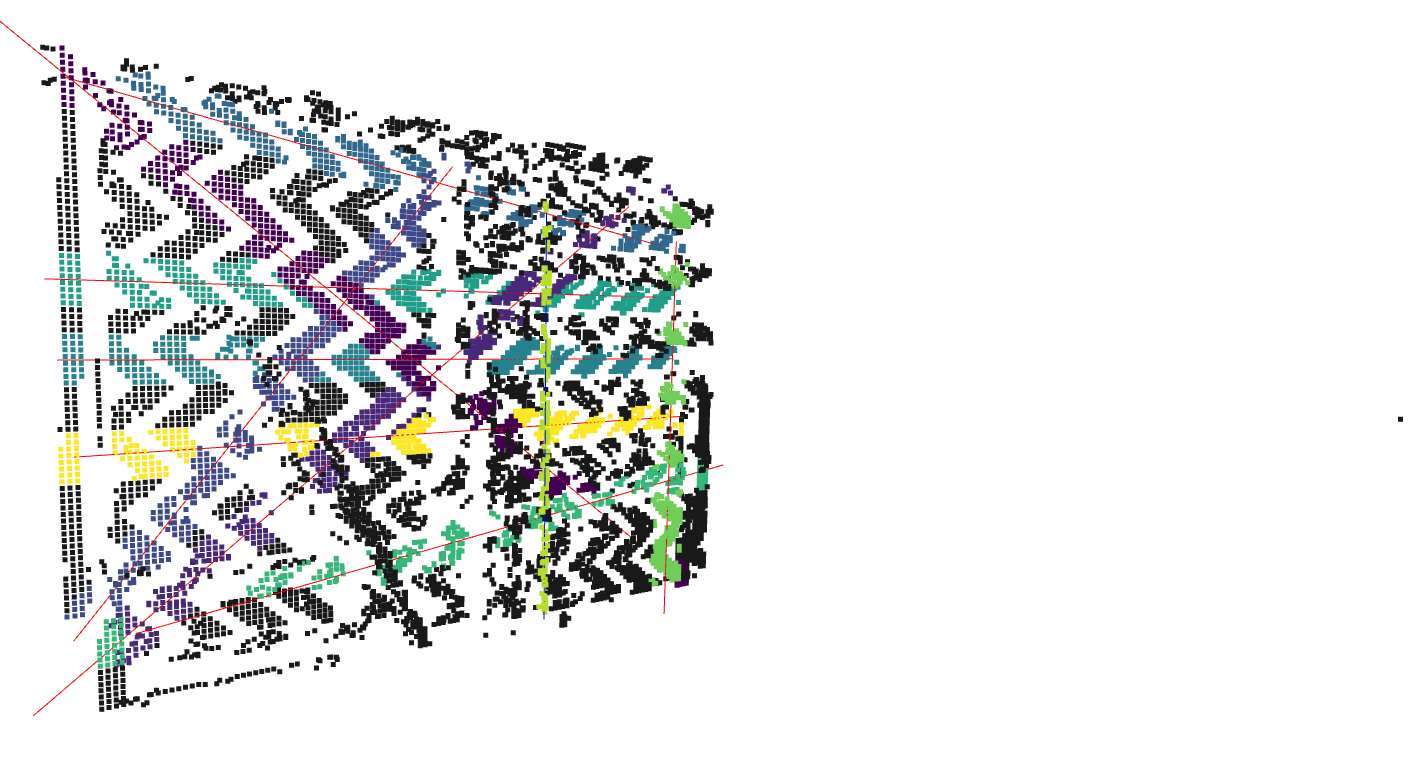
\includegraphics[width=\textwidth]{sections/discussion/zigzag-ptcld-2-obj.png}
    \caption{
        Example of a point cloud display. For each line, the points that belong to it are shown by highlighting
        those points a different color. The lines are also drawn in the point cloud to precisely show their detected
        size and orientation. Only one line is selected as the correct candidate object, and it is drawn in blue. The
        rejected candidate lines are drawn in red. In this example the selected candidate is near the center of the image,
        vertical, and the points belonging to it are shown in lime green. Since it was selected as the correct object,
        its precise size and orientation are shown with a thin blue line passing through the cluster of lime green points.
    }
    \label{fig:ptcld-display}
\end{figure}


\begin{figure}[H]
    \centering
    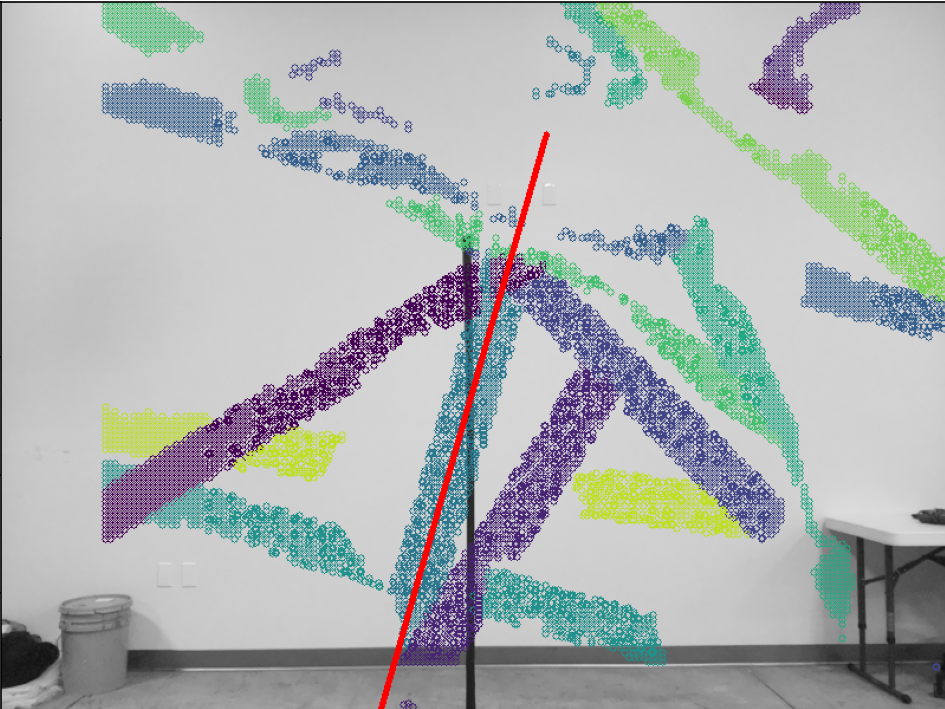
\includegraphics[width=\textwidth]{sections/methods/label_bad_3.png}
    \caption{
        Example of a point cloud overlaid on a grayscale image. Each detected line is shown by projecting the points 
        belonging to it into the 2D image coordinates and highlighting those points a unique color. The line selected
        as the correct object as a solid red line drawn through it showing its precise position and orientation. This
        sample includes many lines that do not correspond to real objects, due to poorly generated disparity data over the 
        textureless backgorund.
    }
    \label{fig:ptcld-overlay}
\end{figure}